% \documentclass[sigconf,review,anonymous]{acmart}
\documentclass[sigconf]{acmart}

\usepackage{booktabs}
\usepackage{multirow}
\usepackage{graphicx}
\usepackage{amsmath}
\usepackage{placeins}
\let\Bbbk\relax  
\usepackage{amssymb}
\usepackage{enumitem}


\settopmatter{printacmref=true}
\settopmatter{printfolios=true}
% \acmSubmissionID{XXX}


\hypersetup{
  pdfinfo={
    Title={GazeMamba: Gaze Trajectory Prediction for Omnidirectional Panoramic Scenes via Hierarchical State-Space Modeling},
  },
  pdfauthor={},
  pdfsubject={ACM MM 2026 Submission},
}


\AtBeginDocument{%
  \providecommand\BibTeX{{%
    Bib\TeX}}}

\copyrightyear{2026}
\acmYear{2026}
\setcopyright{none}
\acmConference[MM '26]{Proceedings of the 34th ACM International Conference on Multimedia}{October 26--30, 2026}{Dublin, Ireland}
\acmDOI{XXXXXXX.XXXXXXX}
\acmISBN{978-1-4503-XXXX-X/26/04}

\begin{document}

\title{GazeMamba: Gaze Trajectory Prediction for Omnidirectional Panoramic Scenes via Hierarchical State-Space Modeling}

\author{Linlin Zhong}
% \email{author1@university.edu}
\affiliation{%
  \institution{East China Normal University}
  \city{Shanghai}
  \country{China}
}

\author{Dandan Zhu}
\authornote{Corresponding author.}
% \email{author2@university.edu}
\affiliation{%
  \institution{East China Normal University}
  \city{Shanghai}
  \country{China}
}

\author{Xiaohui Kong}
% \email{author3@university.edu}
\affiliation{%
  \institution{East China Normal University}
  \city{Shanghai}
  \country{China}
}

\begin{abstract}
Scanpath prediction for 360$^\circ$ omnidirectional images requires modeling the dynamic, ordered gaze behavior of observers freely exploring immersive panoramic content. Existing methods typically fall into two categories: saliency-based samplers that produce temporally incoherent fixation sequences, and first-order Markov generative models that cannot condition on observations more than one step back. We introduce \textbf{GazeMamba}, a framework that pairs a Mamba state-space sequence decoder with a Hierarchical Gaze Sampler HGS and Directional Coordinate Attention DCA. HGS encodes the empirically observed two-phase structure of human visual exploration—an initial broad sweep followed by saliency-focused refinement—as an explicit inductive prior, while DCA decomposes spatial attention into complementary azimuth and elevation encodings suited to the equirectangular panoramic domain. The system is trained end-to-end with a differentiable Soft-DTW alignment objective. Across four 360$^\circ$ benchmarks, Salient360, AOI, JUFE, and Sitzmann, GazeMamba attains state-of-the-art DTW and REC, improving DTW by 14.0\% over the previous best result while using only 1.94\,M parameters, a $6.3\times$ reduction relative to the strongest baseline. The same configuration generalizes zero-shot to unseen datasets and to sequences up to 20\% longer than those seen during training.
\end{abstract}

\begin{CCSXML}
<ccs2012>
   <concept>
       <concept_id>10010147.10010371.10010372</concept_id>
       <concept_desc>Computing methodologies~Image processing</concept_desc>
       <concept_significance>500</concept_significance>
       </concept>
   <concept>
       <concept_id>10010147.10010257.10010293.10010294</concept_id>
       <concept_desc>Computing methodologies~Neural networks</concept_desc>
       <concept_significance>300</concept_significance>
       </concept>
 </ccs2012>
\end{CCSXML}

\ccsdesc[500]{Computing methodologies~Image processing}
\ccsdesc[300]{Computing methodologies~Neural networks}

\keywords{scanpath prediction, 360-degree omnidirectional images, Mamba, hierarchical sampling, coordinate attention, saliency, eye tracking}

\begin{teaserfigure}
  \centering
  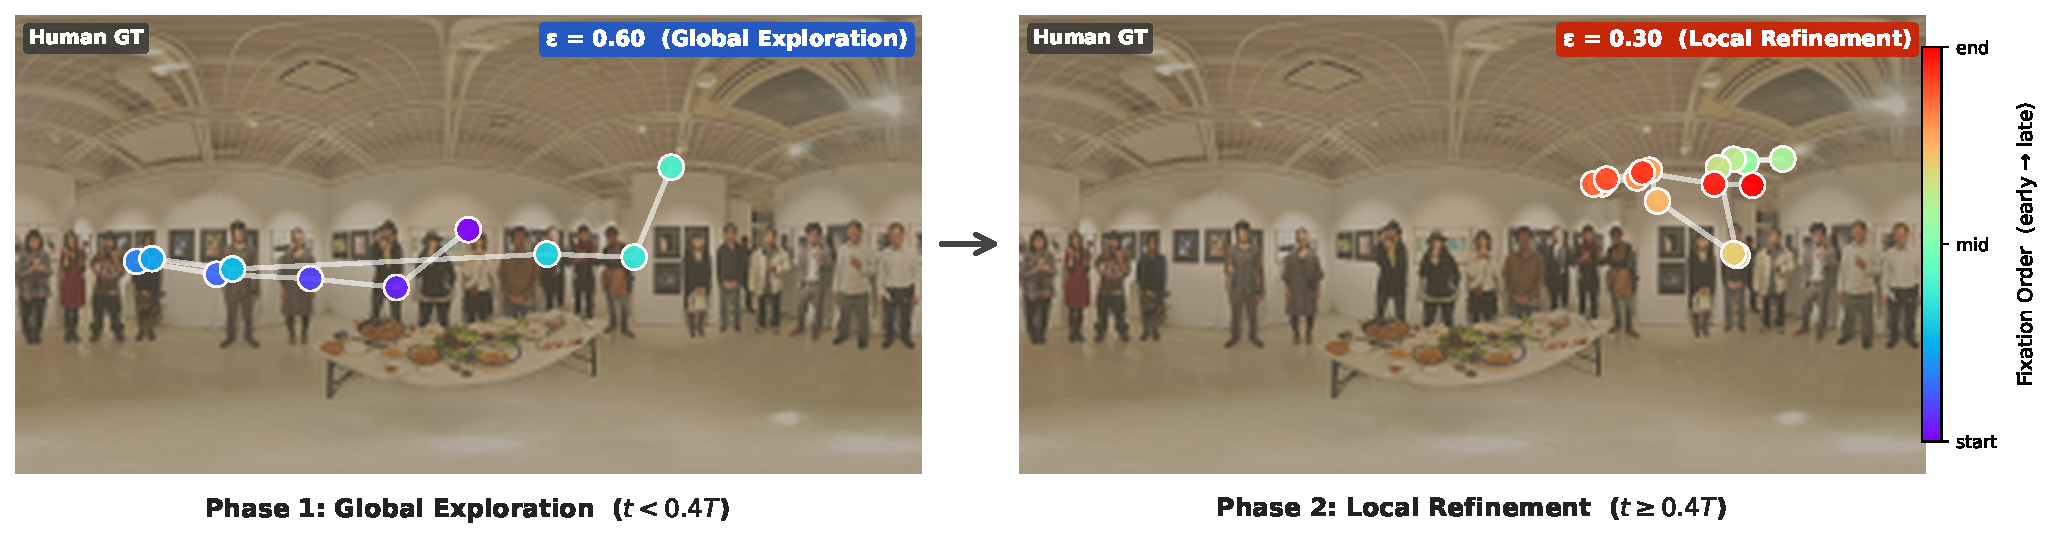
\includegraphics[width=\textwidth]{figures/teaser.pdf}
  \Description{Teaser comparing gaze trajectory predictions from GazeMamba against prior state-of-the-art methods (ScanDMM, ScanGAN, SaltiNet) on three representative 360-degree panoramic scenes, with color-coded fixation sequences overlaid on equirectangular projections.}
  \caption{Qualitative comparison of gaze trajectory predictions from prior state-of-the-art methods and our proposed GazeMamba across three representative 360$^\circ$ panoramic scenes. Unlike saliency-based methods that yield sparse, scattered fixations and deep Markov models that are constrained by first-order temporal dependencies, GazeMamba recovers the two-phase structure of human gaze behavior: an initial broad exploration sweep (blue tones) followed by focused refinement on salient regions (orange tones). Fixation circles are scaled by dwell time; connected saccade arcs encode temporal order from early (blue) to late (orange). DTW scores relative to ground-truth scanpaths are shown in the lower-right of each prediction panel.}
  \label{fig:teaser}
\end{teaserfigure}

\maketitle

% ─────────────────────────────────────────────────────────────────────────────
\section{Introduction}
% ─────────────────────────────────────────────────────────────────────────────

Predicting where and in what order observers look within 360$^\circ$ omnidirectional images is a foundational problem for immersive media systems. Foveated rendering relies on accurate gaze prediction to allocate rendering budget toward attended regions~\cite{swafford2016foveal}; adaptive streaming exploits fixation forecasts to pre-fetch high-quality tiles before the viewer arrives~\cite{petrangeli2018viewport}; and VR interface designers use scanpath models to evaluate spatial layouts and anticipate user confusion~\cite{serrano2017movie}. Unlike conventional 2D images that confine the viewer to a fixed perspective, panoramic scenes invite active head rotation across the full $360^\circ \times 180^\circ$ spherical field of view, demanding temporal gaze models that go well beyond those developed for standard images.

However, predicting human gaze trajectories—commonly known as \emph{scanpath prediction}—is much more challenging for 360$^\circ$ content. Three factors compound this difficulty. First, the equirectangular projection of a panoramic scene introduces pronounced geometric distortion toward the poles, breaking the translational equivariance that standard convolutional architectures rely upon. Second, observers actively rotate their heads to explore the scene, so the dynamics of fixation are shaped not only by the image content but also by vestibular signals, viewing momentum, and prior exploration history. Third, the resulting scanpaths exhibit strong inter-observer variability and non-stationary statistical structure, with distinct behaviors in the early and late phases of a viewing session~\cite{unema2005time,castelhano2009viewing}—a property that demands a temporal representation capable of retaining the full trajectory context rather than merely conditioning on the most recent fixation.

%-- Current landscape and its gaps --%
Existing approaches to 360$^\circ$ scanpath prediction fall into two families. \emph{Saliency-based methods}~\cite{assens2017saltinet,lebreton2018gbvs360} generate fixation sequences by sampling from a static or time-varying saliency map. While conceptually simple, these methods are inherently limited by the quality of the underlying saliency estimator and the design of the sampling heuristic. In practice, the temporal dynamics they produce are often physically implausible—characterized by large inter-fixation displacements and sparse coverage of semantically interesting regions, as illustrated in Figure~\ref{fig:teaser}. \emph{Generative methods} address some of these shortcomings by learning to synthesize realistic trajectories from data. GAN-based approaches~\cite{martin2022scangan} produce diverse scanpaths but are prone to training instability and struggle to generate sequences of variable length. ScanDMM~\cite{sui2023scandmm} is a strong recent baseline that frames scanpath prediction as inference in a Deep Markov Model, maintaining a latent visual state $\mathbf{z}_t$ that encodes the evolving attentional landscape. However, the first-order Markov structure of DMM constrains each state transition to depend only on the immediately preceding state $\mathbf{z}_{t-1}$, making it impossible to condition fixation predictions on observations from many steps earlier—a significant limitation given that human inhibition of return operates over multi-fixation timescales. Furthermore, the variational Evidence Lower Bound objective introduces substantial training complexity through KL annealing and posterior approximation. To the best of our knowledge, none of the above methods fully captures the temporal dependency structure of human gaze behavior in panoramic scenes.

%-- The missing ingredient: two-phase structure --%
A recurring observation in the eye-tracking literature is that human gaze exploration of novel scenes follows a characteristic \emph{two-phase} progression~\cite{unema2005time}. In the early phase, fixations are broadly distributed, sweeping across the scene to rapidly form a gist-level representation. In the later phase, attention converges toward semantically salient regions for detailed inspection. This global-to-local organization is consistent across observers and scene types, yet no prior scanpath prediction method for 360$^\circ$ images explicitly encodes it as a structural inductive prior, leaving a gap between model assumptions and the actual temporal dynamics of human gaze.

To this end, we propose GazeMamba, a scanpath prediction framework built around three components. The Hierarchical Gaze Sampler divides the fixation sequence into a broad exploration phase and a focused refinement phase, each governed by a distinct sampling policy with phase-specific exploration rates and saliency guidance. Momentum smoothing within each phase encourages physically plausible saccade amplitudes and smooth gaze transitions. Directional Coordinate Attention is applied in both the global panoramic encoder and the local patch encoder. It decomposes spatial attention into independent horizontal and vertical 1D encodings that localize salient content along the azimuth and elevation axes, directions that carry distinct semantic meaning in equirectangular panoramas. A Mamba state-space sequence decoder replaces the first-order Markov chain of prior work with a selective state-space model that conditions each fixation prediction on the full preceding trajectory through content-dependent gating, while retaining linear-time computation instead of the quadratic cost of self-attention. The entire framework is trained end-to-end with a differentiable Soft-DTW sequence alignment loss, avoiding the complexity of variational objectives.

Our contributions are as follows.
\begin{enumerate}[topsep=2pt,itemsep=2pt]
  \item We propose a \textbf{Hierarchical Gaze Sampler} that explicitly encodes the two-phase structure of human visual exploration in 360$^\circ$ panoramic scenes, combining phase-specific exploration rates with momentum smoothing to produce smooth and spatially diverse gaze trajectories.
  \item We introduce \textbf{Directional Coordinate Attention}, a lightweight attention module that decomposes spatial context into azimuth and elevation encodings, enabling both global and local visual encoders to precisely localize salient content in wide-format equirectangular projections.
  \item We present a \textbf{Mamba-based gaze trajectory decoder} that models long-range fixation dependencies through selective state-space updates, overcoming the first-order Markov bottleneck of existing deep generative scanpath models while maintaining linear inference complexity.
  \item Extensive experiments on four 360$^\circ$ scanpath benchmarks demonstrate state-of-the-art DTW and REC performance and strong zero-shot generalization across unseen datasets and sequence lengths. In Salient360, GazeMamba improves DTW by \textbf{14.0\%} over the prior state of the art while using $6.3\times$ fewer parameters than the strongest baseline, indicating that accuracy and efficiency can be achieved simultaneously.
\end{enumerate}

\section{Related Work}

\textbf{Saliency Prediction for Panoramic Images.} Visual saliency prediction has evolved from early bottom-up models based on low-level features~\cite{itti1998saliency} to deep learning architectures~\cite{li2016deepcontrast,wang2017salientobject}. Extensions to 360$^\circ$ imagery handle spherical distortion via graph-based representations~\cite{lv2020salgcn,chen2020salbinet360} or geometry-aware vision Transformers that process tangent-plane patches with spherical positional encodings~\cite{cokelek2024salvit360}. While saliency maps characterize \emph{where} observers look in aggregate, they discard the temporal ordering of fixations and thus cannot directly serve as scanpath predictions; bridging this gap motivates the scanpath prediction approaches reviewed below.
\vspace{1em}

\noindent\textbf{Scanpath Prediction .}Early scanpath models drew on probabilistic gaze dynamics and saccadic decision theory~\cite{boccignone2004randomwalk}. Subsequent deep learning methods achieved strong performance through RNN-based mixture density networks~\cite{sun2021iorroi,wolfe2021guidedsearch}, multi-observer sequence generators~\cite{debelan2022scanpathnet}, and unified fixation-and-scanpath predictors~\cite{kummerer2022deepgazeIII}. For 360$^\circ$ content, PathGAN~\cite{martin2022scangan} adapted adversarial generation to the spherical domain using S-CNN and CoordConv layers. ScanDMM~\cite{sui2023scandmm} introduced a Deep Markov Model with semantic-guided state transitions. PathFormer3D~\cite{quan2024pathformer3d} extends Transformer-based trajectory modeling to the 360$^\circ$ domain by incorporating 3D spherical positional encodings and cross-attention between local patch tokens and a scene-level saliency context, at the cost of substantial model complexity. Neural temporal point processes~\cite{damelio2024tppgaze} and few-shot personalization techniques~\cite{xue2024fewshot} extend scanpath modeling to duration prediction and individual-level gaze behavior. HAT~\cite{yang2024unify} unifies top-down task guidance and bottom-up saliency within a single Transformer framework and shows strong performance on task-driven scanpath datasets; it is however designed for 2D images and does not address the geometric distortions or directional asymmetry of equirectangular panoramas. Diffusion-based methods~\cite{cartella2025scandiff} use stochastic denoising to generate diverse, realistic trajectories. ScanDTM~\cite{zhu2025scandtm} combines a Dual-GCN encoder with a diffusion-guided saliency module for strong cross-dataset generalization, but its graph-construction preprocessing and iterative diffusion sampling make real-time inference impractical, and no public implementation currently permits reproduction on all four benchmarks we evaluate. Within this landscape, GazeMamba combines a Mamba state-space backbone with an explicit two-phase hierarchical sampling prior, achieving superior trajectory accuracy with substantially lower model complexity. The design addresses three gaps left by existing work: long-range trajectory context is handled by the Mamba decoder, global-to-local exploration by HGS, and directional asymmetry of equirectangular panoramas by DCA in both encoders.

% \textbf{State Space Models and Spatial Attention. }Structured State Space Sequences (S4)~\cite{gu2021efficiently} demonstrated that continuous-time state-space parameterizations can capture long-range dependencies in sequences of extreme length. Mamba~\cite{gu2023mamba} extended this family with data-dependent selective state transitions, matching Transformer accuracy at linear computational cost; Vision Mamba~\cite{zhu2024vision} demonstrated its effectiveness for 2D image recognition. Coordinate Attention~\cite{hou2021coordinate} decomposes channel recalibration into horizontal and vertical 1D encodings, preserving positional context that global pooling discards. To the best of our knowledge—based on a systematic search of arXiv, IEEE Xplore, and ACM DL conducted in March 2026—GazeMamba is among the first models to apply a Mamba backbone to scanpath prediction and to pair it with direction-aware coordinate attention specifically designed for the equirectangular panoramic domain.

% ─────────────────────────────────────────────────────────────────────────────
\section{Method}
% ─────────────────────────────────────────────────────────────────────────────

\begin{figure*}[t]
  \centering
  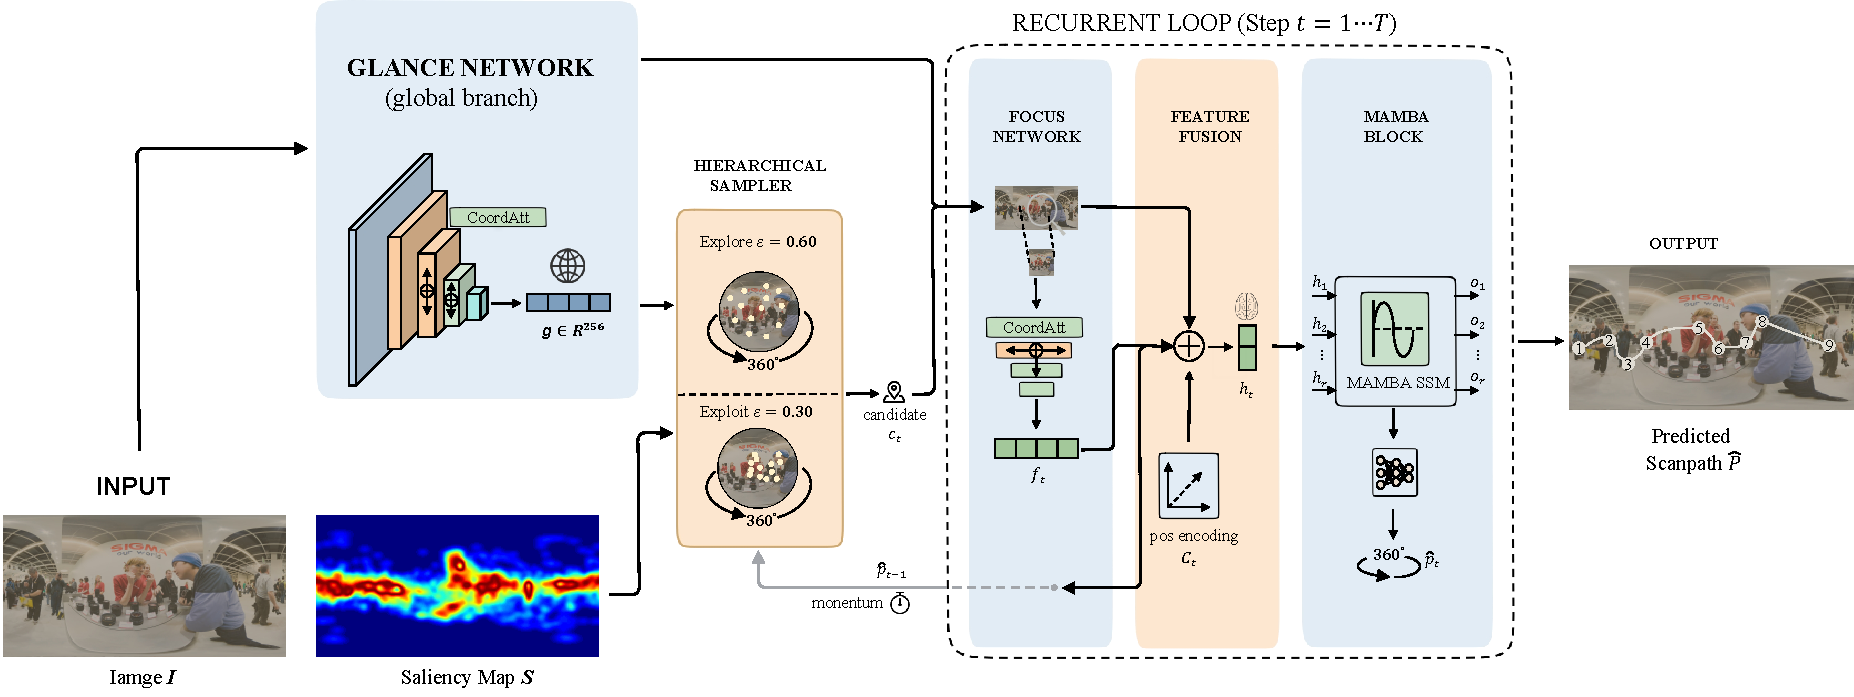
\includegraphics[width=\textwidth]{figures/architecture.pdf}
  \Description{Overall architecture diagram of GazeMamba, illustrating the panoramic scene encoder with Directional Coordinate Attention, the Hierarchical Gaze Sampler with its two-phase exploration schedule, the local patch encoder, the Mamba sequence decoder, and the Soft-DTW training objective.}
  \caption{Overall architecture of \textbf{GazeMamba}. Given a 360$^\circ$ panoramic image $\mathbf{I}$ and its saliency map $\mathbf{S}$, the \emph{Scene Encoder} extracts a global context vector $\mathbf{g}$ using Directional Coordinate Attention. At each step $t$, the \emph{Hierarchical Gaze Sampler HGS} draws a candidate fixation $\mathbf{c}_t$ according to the current phase policy; the \emph{Patch Encoder} extracts a local feature $\mathbf{f}_t$ from the corresponding image region; and the combined token $\mathbf{h}_t$ is processed by the \emph{Mamba Gaze Decoder} to predict the refined fixation coordinate $\hat{\mathbf{p}}_t$. The framework is trained end-to-end with a Soft-DTW alignment loss augmented by a panoramic coverage regularizer.}
  \label{fig:architecture}
\end{figure*}

\subsection{Problem Formulation}
Given a 360$^\circ$ panoramic image $\mathbf{I} \in \mathbb{R}^{3 \times H \times W}$ and its saliency map $\mathbf{S} \in \mathbb{R}^{1 \times H \times W}$, we aim to predict a scanpath $\hat{\mathbf{P}} = \{(\hat{x}_t, \hat{y}_t)\}_{t=1}^{T}$, where each $(\hat{x}_t, \hat{y}_t) \in [0,1]^2$ denotes a normalized fixation coordinate in the equirectangular projection. We model scanpath generation as sampling from a conditional distribution
\begin{equation}
  p_\theta(\hat{\mathbf{P}} \mid \mathbf{I}, \mathbf{S})
  = \prod_{t=1}^{T} p_\theta(\hat{\mathbf{p}}_t \mid \hat{\mathbf{p}}_{<t}, \mathbf{I}, \mathbf{S}),
  \label{eq:cond_factorization}
\end{equation}
where $\hat{\mathbf{p}}_t = (\hat{x}_t, \hat{y}_t)$ denotes the $t$-th fixation and $\hat{\mathbf{p}}_{<t} = \{\hat{\mathbf{p}}_1,\dots,\hat{\mathbf{p}}_{t-1}\}$ denotes the fixation history. In practice, we first map $(\mathbf{I}, \mathbf{S}, \hat{\mathbf{p}}_{<t})$ into a sequence of latent tokens
\begin{equation}
  \mathbf{H}
  = \bigl(\mathbf{h}_1,\dots,\mathbf{h}_T\bigr)
  = \Phi_\theta(\mathbf{I}, \mathbf{S}, \hat{\mathbf{p}}_{<1:T}),
\end{equation}
where $\Phi_\theta$ denotes the composition of the scene encoder, patch encoder, and HGS. The Mamba decoder then produces a context vector at each step, and the conditional in~\eqref{eq:cond_factorization} can be written as
\begin{equation}
  p_\theta(\hat{\mathbf{p}}_t \mid \hat{\mathbf{p}}_{<t}, \mathbf{I}, \mathbf{S})
  = p_\theta\bigl(\hat{\mathbf{p}}_t \mid \mathrm{Mamba}_\theta(\mathbf{H})_t\bigr).
\end{equation}
GazeMamba thus realizes~\eqref{eq:cond_factorization} through a sequence of learned latent representations and content-dependent state-space updates.

\subsection{Scene Encoder}
The Scene Encoder $\mathcal{G}$ extracts a global panoramic representation from the full equirectangular image. Before directing attention to any specific location, observers rapidly form a holistic impression of the scene layout—the so-called ``gist''—that shapes subsequent fixation decisions. Capturing this scene-level context grounds all subsequent fixation predictions in a coherent global representation. The encoder comprises a lightweight convolutional backbone with two DCA modules inserted after the second and third convolutional stages:

\begin{figure}[b]
  \centering
  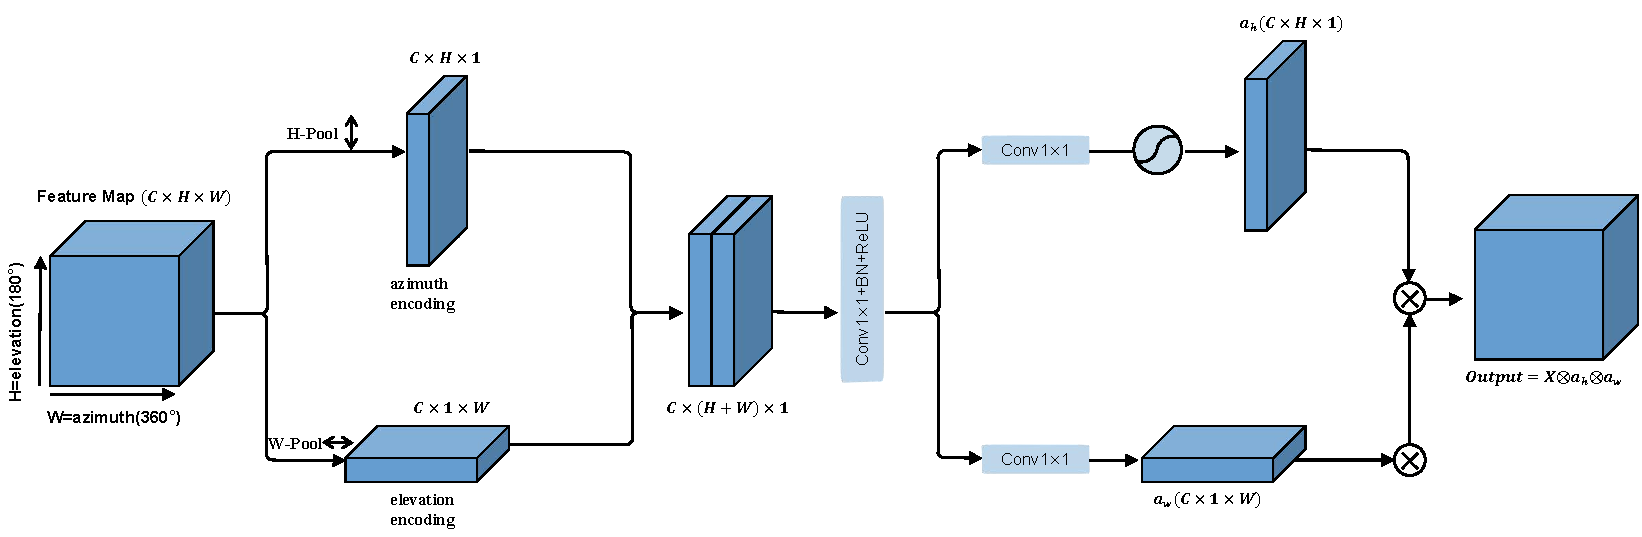
\includegraphics[width=0.9\linewidth]{figures/coordatt.pdf}
  \Description{Three-panel illustration of Directional Coordinate Attention. Left: equirectangular projection asymmetry with azimuth and elevation axes. Middle: the DCA module with separate azimuth and elevation pooling branches, a shared projection, and direction-specific attention weights. Right: visualization of azimuth and elevation attention maps on a sample panorama, together with the DTW degradation observed when DCA is removed.}
  \caption{\textbf{Directional Coordinate Attention}. Left: equirectangular projection asymmetry, where horizontal azimuth and vertical elevation encode different semantic structures that standard isotropic attention cannot distinguish. Middle: the DCA module takes a feature map $\mathbf{X} \in \mathbb{R}^{C \times H \times W}$, applies azimuth-wise and elevation-wise pooling, concatenates the resulting 1D embeddings, and passes them through a shared Conv$1{\times}1$ to produce direction-aware attention weights $a_h$ and $a_w$. Right: azimuth and elevation attention maps on a sample panorama, whose combination yields a directionally aware response; removing DCA increases DTW by 2.9\%.}
  \label{fig:coordatt}
\end{figure}

\begin{equation}
  \mathbf{g} = \mathcal{G}(\mathbf{I}) \in \mathbb{R}^{d},
\end{equation}
where $d = 256$ is the feature dimension. DCA decomposes attention into horizontal (azimuth) and vertical (elevation) pooling branches, producing spatially sensitive channel weights that capture the directional semantics of wide-format panoramic images. The key property of this design is that it preserves the asymmetry between azimuth and elevation: the horizontal extent of an equirectangular panorama is twice the vertical, and the distribution of salient content along each axis has a different structure that a single isotropic attention mechanism cannot distinguish.

\subsection{Patch Encoder}
While the Scene Encoder captures global context, local patch features capture the fine-grained visual content at each candidate fixation location. At each step $t$, the Patch Encoder $\mathcal{F}$ extracts a local representation from a patch centered at the current fixation position $\mathbf{p}_t = (x_t, y_t)$. During training, $\mathbf{p}_t$ is the scheduled-sampling input (ground-truth fixation with probability $r_t$, previous model prediction otherwise); at inference, it is the model's own most recent prediction.
\begin{equation}
  \mathbf{f}_t = \mathcal{F}(\mathbf{I}, \mathbf{p}_t) \in \mathbb{R}^{d},
\end{equation}
where the patch is extracted with spatial extent $\min(H,W)/4$ and resized to $64 \times 64$ via bilinear interpolation, providing a consistent local context window independent of image resolution. A DCA module after the second convolutional stage preserves directional structure within the patch, retaining spatial relationships within locally attended regions.

\subsection{Hierarchical Gaze Sampler}
\label{sec:sampler}

Human visual exploration of panoramic scenes follows a consistent hierarchical pattern: early fixations sweep broadly to construct a scene-level gist representation, while later fixations converge on locally salient regions for detailed inspection~\cite{unema2005time,castelhano2009viewing}. This global-to-local organization mirrors the coarse-to-fine processing hierarchy observed across perceptual and cognitive systems~\cite{castelhano2009viewing}, and is analogous to the two-stage visual acquisition strategy employed by active vision models: a broad ambient phase establishes scene structure, followed by a focal phase that directs fine-grained analysis toward high-priority locations. We instantiate this prior as a \emph{two-phase} sampling strategy that explicitly encodes the temporal structure of gaze behavior, as illustrated in Figure~\ref{fig:sampler}.

\begin{figure}[t]
  \centering
  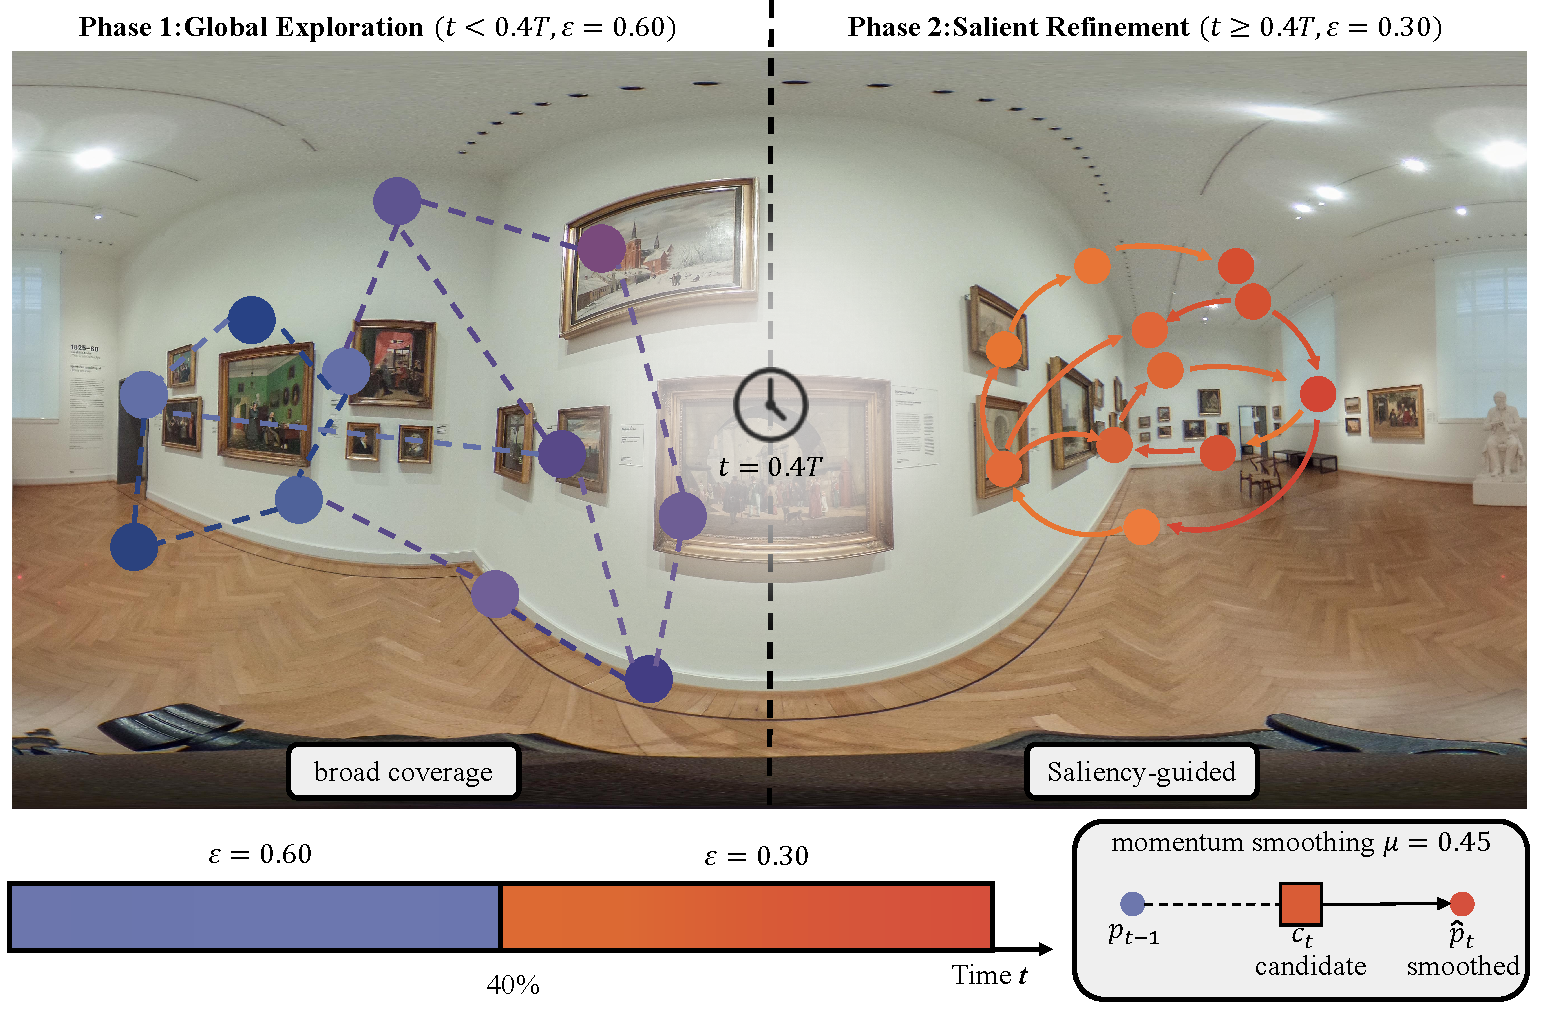
\includegraphics[width=\linewidth]{figures/sampler.pdf}
  \Description{Diagram of the Hierarchical Gaze Sampler showing Phase 1 (high-exploration, broad spatial coverage) and Phase 2 (low-exploration, concentrated on salient regions) with momentum-smoothed transitions between fixations.}
  \caption{\textbf{Hierarchical Gaze Sampler HGS}. Phase~1 ($t < 0.4T$, $\varepsilon_1{=}0.60$) distributes fixations broadly across the panorama to establish scene coverage; Phase~2 ($t \geq 0.4T$, $\varepsilon_2{=}0.30$) concentrates sampling on high-saliency regions. Momentum smoothing enforces physically plausible inter-fixation transitions.}
  \label{fig:sampler}
\end{figure}

Formally, at step $t$ we draw a phase-conditioned exploration indicator $z_t \in \{0,1\}$:
\begin{equation}
  z_t \sim \mathrm{Bernoulli}\bigl(\varepsilon(t)\bigr), \qquad
  \varepsilon(t) =
  \begin{cases}
    \varepsilon_1 & \text{if } t < \alpha T, \\
    \varepsilon_2 & \text{otherwise,}
  \end{cases}
  \label{eq:hgs_eps}
\end{equation}
where $\alpha = 0.4$ is the phase transition ratio and $T$ is the total sequence length. The elevated exploration rate $\varepsilon_1$ in Phase~1 prevents premature attentional collapse, while the reduced rate $\varepsilon_2$ in Phase~2 concentrates fixations on semantically salient regions consistent with ground-truth distributions.

Conditioned on $z_t$, the candidate fixation $\mathbf{c}_t$ is sampled from a mixture distribution
\begin{equation}
  p(\mathbf{c}_t \mid \mathbf{S}, \mathbf{p}_{t-1})
  = \varepsilon(t)\,\mathcal{U}([0,1]^2)
    + \bigl(1 - \varepsilon(t)\bigr)\,p_{\text{sal}}(\mathbf{c}_t \mid \mathbf{S}, \mathbf{p}_{t-1}),
  \label{eq:hgs_mixture}
\end{equation}
where $\mathcal{U}([0,1]^2)$ is a uniform distribution over the normalized panorama and $p_{\text{sal}}$ denotes a saliency-biased kernel obtained from $\mathrm{softmax}(\mathbf{S}/\tau)$ followed by momentum smoothing. Concretely, letting $\tilde{\mathbf{c}}_t$ be a position sampled from the saliency map with temperature $\tau = 0.12$, we update
\begin{equation}
  \mathbf{c}_t
  = (1-\mu)\,\tilde{\mathbf{c}}_t
    + \mu \bigl(\mathbf{p}_{t-1} + \delta_{t-1} s_{\max}\bigr),
  \label{eq:hgs_momentum}
\end{equation}
where $\mu = 0.45$ is the momentum coefficient, $\delta_{t-1}$ is the unit direction vector of the previous saccade, and $s_{\max} = 0.18$ is the maximum allowable step size. A hard displacement constraint then enforces $\|\mathbf{c}_t - \mathbf{p}_{t-1}\| \le s_{\max}$, preventing saccade amplitudes from exceeding the physiologically plausible range.

\subsection{Mamba Gaze Decoder}
The sampler provides candidate fixation positions, but the final prediction must integrate global context, local visual content, and full positional history to produce accurate fixation coordinates. At each step $t$, we form a unified feature token by combining the global scene representation, the local patch feature, and a positional encoding of the candidate fixation:
\begin{equation}
  \mathbf{h}_t = \mathbf{g} + \mathbf{f}_t + \mathrm{MLP}_{\mathrm{pos}}(\mathbf{p}_t),
\end{equation}
where $\mathrm{MLP}_{\mathrm{pos}}$ is a two-layer MLP that projects the 2D coordinate into the $d$-dimensional feature space. The token sequence $\{\mathbf{h}_t\}_{t=1}^{T}$ is processed by a Mamba block configured with $d_{\mathrm{model}}=256$, $d_{\mathrm{state}}=256$, $d_{\mathrm{conv}}=4$, and an expansion factor of 2.

Concretely, Mamba discretizes a continuous SSM with learnable step size $\Delta_t$, state transition matrix $\mathbf{A}$, and input-dependent projection matrices $\mathbf{B}_t, \mathbf{C}_t$ that are computed from $\mathbf{h}_t$:
\begin{equation}
  \mathbf{s}_t = \bar{\mathbf{A}}_t\,\mathbf{s}_{t-1} + \bar{\mathbf{B}}_t\,\mathbf{h}_t, \qquad
  \mathbf{o}_t = \mathbf{C}_t\,\mathbf{s}_t,
\end{equation}
where $\bar{\mathbf{A}}_t = \exp(\Delta_t \mathbf{A})$ and $\bar{\mathbf{B}}_t = (\Delta_t \mathbf{A})^{-1}(\bar{\mathbf{A}}_t - \mathbf{I})\,\mathbf{B}_t$ are the discretized parameters. Because $\mathbf{B}_t$ and $\mathbf{C}_t$ depend on the current input, the state update is \emph{content-selective}: at each fixation step, only context relevant to the current candidate position influences the hidden state $\mathbf{s}_t$, while irrelevant prior fixations are attenuated. This provides a principled, implicit inhibition-of-return mechanism that propagates long-distance fixation dependencies without the quadratic memory cost of self-attention. Let $\mathbf{H} = (\mathbf{h}_1, \ldots, \mathbf{h}_T) \in \mathbb{R}^{T \times d}$ denote the full token matrix; the refined fixation coordinate is produced by a sigmoid-activated two-layer MLP:
\begin{equation}
  \hat{\mathbf{p}}_t = \sigma(\mathrm{MLP}_{\mathrm{dec}}(\mathrm{Mamba}(\mathbf{H})_t)).
\end{equation}

\subsection{Training Objective}
Given a training set $\mathcal{D} = \{(\mathbf{I}^{(n)}, \mathbf{S}^{(n)}, \mathbf{P}^{*(n)})\}_{n=1}^{N}$, we minimize the empirical risk
\begin{equation}
  \mathcal{J}(\theta)
  = \frac{1}{N} \sum_{n=1}^{N}
    \Bigl[
      \mathcal{L}_{\mathrm{traj}}\bigl(\hat{\mathbf{P}}^{(n)}, \mathbf{P}^{*(n)}\bigr)
      + \lambda\,\mathcal{L}_{\mathrm{cov}}\bigl(\hat{\mathbf{P}}^{(n)}\bigr)
    \Bigr],
  \label{eq:empirical_risk}
\end{equation}
where $\hat{\mathbf{P}}^{(n)}$ is sampled from $p_\theta(\hat{\mathbf{P}} \mid \mathbf{I}^{(n)}, \mathbf{S}^{(n)})$ and $\lambda$ balances trajectory accuracy and coverage.

Standard point-wise regression losses treat fixations independently and are insensitive to temporal ordering. We instead adopt Soft-DTW~\cite{cuturi2017soft}, a differentiable relaxation of dynamic time warping that measures the minimum-cost temporal alignment between predicted and ground-truth sequences:
\begin{equation}
  \mathcal{L}_{\mathrm{traj}}(\hat{\mathbf{P}}, \mathbf{P}^*) = \mathrm{SoftDTW}_\gamma(\hat{\mathbf{P}}, \mathbf{P}^*),
\end{equation}
with smoothing parameter $\gamma = 0.10$. Writing $\hat{\mathbf{P}} = \{\hat{\mathbf{p}}_i\}_{i=1}^{T}$ and $\mathbf{P}^* = \{\mathbf{p}^*_j\}_{j=1}^{T^*}$, Soft-DTW can be expressed as
\begin{equation}
  \mathrm{SoftDTW}_\gamma(\hat{\mathbf{P}}, \mathbf{P}^*)
  = -\gamma \log \sum_{\boldsymbol{\pi} \in \Pi}
      \exp\!\left(
        - \frac{1}{\gamma}
          \sum_{(i,j) \in \boldsymbol{\pi}}
            \bigl\|\hat{\mathbf{p}}_i - \mathbf{p}^*_j\bigr\|_2
      \right),
\end{equation}
where $\Pi$ is the set of all monotone alignment paths between the two sequences. The smoothing parameter $\gamma$ controls the sharpness of the soft minimum over paths: as $\gamma \to 0$, $\mathcal{L}_{\mathrm{traj}}$ approaches hard DTW, while larger $\gamma$ yields a smoother objective that still provides informative gradients when predictions are poorly aligned during early training.

An auxiliary panoramic coverage regularizer discourages degenerate solutions in which all predicted fixations collapse to a narrow region of the panorama:
\begin{equation}
  \mathcal{L}_{\mathrm{cov}}(\hat{\mathbf{P}}) = -\!\left(w_x\,(\sigma_x + r_x) + w_y\,(\sigma_y + r_y)\right),
\end{equation}
where $\sigma_x, r_x$ are the standard deviation and range of predicted $x$-coordinates across the sequence, and $w_x=2.0$, $w_y=1.0$ reflect the 2:1 aspect ratio of equirectangular projections. The negative sign means a lower loss corresponds to higher spatial spread, penalizing collapsed trajectories.

Scheduled sampling with exponential decay is used during training: at step $t$, the ground-truth fixation is fed as input with probability $r_t = 0.8 \times 0.95^t$, and the model's own prediction is used otherwise. This curriculum gradually shifts training from full teacher forcing toward free-running inference, preventing the model from becoming dependent on ground-truth context at test time.

% ─────────────────────────────────────────────────────────────────────────────
\FloatBarrier
\section{Experiments}
% ─────────────────────────────────────────────────────────────────────────────

\subsection{Datasets}
We evaluate on four 360$^\circ$ scanpath benchmarks:

\textbf{Salient360} contains 85 equirectangular panoramas with free-viewing scanpaths from multiple observers. We use the official train/test split (272/17 scanpath instances), with sequence length $T=25$. This dataset serves as the primary training and in-distribution evaluation benchmark.

\textbf{AOI} comprises 384 panoramic images with 9-fixation scanpaths. Its short sequences make it a useful probe for cross-dataset generalization under conditions where each trajectory is too brief for long-range temporal dependencies to dominate.

\textbf{JUFE} includes 1800 panoramic images with 15-fixation scanpaths collected under a focused-attention paradigm, where observers concentrated on specific task-relevant regions rather than freely exploring the scene. Spherical coordinates are converted to normalized equirectangular coordinates via longitude--latitude projection. This dataset tests generalization to task-driven gaze behavior that differs from the free-viewing training data.

\textbf{Sitzmann} contains 48 high-resolution panoramas with 30-fixation scanpaths, providing a stress test for sequence-length generalization since all training was done with $T=25$.

\subsection{Evaluation Metrics}
We adopt three established scanpath comparison metrics~\cite{fahimi2021scanpathmetrics,bylinskii2019metrics}:

\textbf{Levenshtein Distance (LEV)}: Edit distance between discretized scanpath strings on a $12 \times 8$ grid. Lower is better.

\textbf{Dynamic Time Warping (DTW)}: Minimum-cost temporal alignment between predicted and ground-truth fixation sequences using Euclidean distance. Lower is better.

\textbf{Recurrence Rate (REC)}: Cross-recurrence between predicted and ground-truth fixations within a 12-pixel threshold. Higher is better.

The \textbf{Human upper bound} in Table~\ref{tab:sota} is computed via leave-one-out cross-observer evaluation: for each scanpath in the test set, one observer's sequence is treated as the ``prediction'' and the mean metric against all remaining observers' sequences on the same image is reported as the upper bound. This provides a principled estimate of inter-observer agreement under the same metrics used for automatic methods.

\subsection{Implementation Details}
All models are implemented in PyTorch and optimized with AdamW ($\text{lr}=10^{-4}$, weight decay $10^{-4}$) for 50 epochs with cosine annealing. Batch size is 128; images are resized to $128 \times 256$. Training uses the Salient360 training split only (272 scanpath instances); all remaining datasets—including JUFE (1800 images, ${\approx}7\times$ more data)—are evaluated \emph{zero-shot} without any fine-tuning or domain adaptation. This strict zero-shot protocol is intentional: our goal is to assess whether the structural inductive priors encoded by HGS and DCA confer cross-domain generalization, rather than fitting to each benchmark individually. Experiments are conducted on a single GPU (NVIDIA A100). All ablation results are averaged over 3 independent runs with different random seeds (0, 1, 2); run-to-run standard deviations were below $\pm0.4$ on LEV, $\pm35$ on DTW, and $\pm0.35$ on REC across all variants, confirming result stability. Code and trained model checkpoints will be released upon publication.

\subsection{Comparison with State-of-the-Art}
\label{sec:sota}

\begin{table*}[t]
  \centering
  \caption{Quantitative comparison on four 360$^\circ$ scanpath benchmarks. AOI, JUFE, and Sitzmann are evaluated in a zero-shot setting (no fine-tuning). $\downarrow$: lower is better; $\uparrow$: higher is better. Best results in \textbf{bold}. $^\ddagger$GazeMamba ranks second on AOI LEV (13.06 vs.\ ScanDMM 12.13); see §\ref{sec:sota} for analysis. Human upper bound is shown for reference.}
  \label{tab:sota}
  \setlength{\tabcolsep}{4.5pt}
  \begin{tabular}{lcccccccccccc}
    \toprule
    & \multicolumn{3}{c}{Salient360} & \multicolumn{3}{c}{AOI} & \multicolumn{3}{c}{JUFE} & \multicolumn{3}{c}{Sitzmann} \\
    \cmidrule(lr){2-4}\cmidrule(lr){5-7}\cmidrule(lr){8-10}\cmidrule(lr){11-13}
    Method & LEV$\downarrow$ & DTW$\downarrow$ & REC$\uparrow$ & LEV$\downarrow$ & DTW$\downarrow$ & REC$\uparrow$ & LEV$\downarrow$ & DTW$\downarrow$ & REC$\uparrow$ & LEV$\downarrow$ & DTW$\downarrow$ & REC$\uparrow$ \\
    \midrule
    CLE           & 39.77 & 1714.4 & 3.32 & 12.87 & 547.9 & 3.62 & 24.84 & 1172.2 & 3.01 & 45.18 & 1967.3 & 3.13 \\
    DeepGazeIII   & 40.01 & 1742.4 & 2.59 & 13.16 & 558.5 & 2.89 & 24.13 & 1104.9 & 2.77 & 46.42 & 1992.9 & 3.08 \\
    SaltiNet      & 40.85 & 1855.5 & 2.31 & 14.70 & 596.5 & 2.24 & 26.07 & 1287.1 & 1.54 & 51.37 & 2305.1 & 1.56 \\
    ScanGAN       & 38.93 & 1721.7 & 3.10 & 12.89 & 552.5 & 3.75 & 24.21 & 1095.0 & 3.08 & 45.27 & 1951.9 & 3.24 \\
    ScanDMM       & 37.27 & 1528.6 & 3.58 & 12.13 & 537.5 & 4.02 & 23.09 & 1086.0 & 4.33 & 44.97 & 1965.4 & 3.48 \\
    HAT           & 36.14 & 1520.1 & 4.17 & 13.65 & 522.2 & 5.32 & 22.74 & 1087.2 & 3.94 & 44.10 & 1960.6 & 3.95 \\
    PathFormer3D  & 36.28 & 1515.9 & 4.25 & 13.90 & 561.9 & 8.29 & 22.60 & 1054.2 & 4.45 & 44.69 & 1939.7 & 4.15 \\
    Human         & 35.08 & 1382.6 & 5.20 & 9.24  & 389.5 & 6.23 & 18.31 & 1038.9 & 7.75 & 41.19 & 1837.0 & 6.35 \\
    \midrule
    \textbf{GazeMamba} & \textbf{36.07} & \textbf{1305.0} & \textbf{5.58} & 13.06 & \textbf{468.2} & \textbf{6.52} & \textbf{21.61} & \textbf{1059.6} & \textbf{5.21} & \textbf{38.12} & \textbf{1524.9} & \textbf{4.19} \\
    \bottomrule
  \end{tabular}
\end{table*}

\textbf{Accuracy Comparison.} Table~\ref{tab:sota} reports the quantitative results. Baselines include CLE (Center-biased Location Estimate: fixations sampled from a Gaussian centered at the equirectangular midpoint, capturing the well-documented equator bias~\cite{assens2018scanpath360}), DeepGazeIII, SaltiNet, ScanGAN, ScanDMM, and PathFormer3D. Across all four benchmarks, GazeMamba attains the lowest DTW scores and the highest REC scores among all evaluated methods. On Salient360, DTW improves over the prior best (PathFormer3D: 1515.9) by \textbf{14.0\%} (1305.0), and GazeMamba also achieves the lowest LEV (36.07) among automatic methods, within one edit-distance unit of the human upper bound (35.08). On JUFE, GazeMamba leads on both LEV (21.61) and DTW (1059.6), confirming that the learned viewing strategy transfers to task-driven gaze behavior. On Sitzmann—sequences 20\% longer than training ($T{=}30$ vs.\ $T{=}25$)—GazeMamba achieves the best DTW (1524.9) and REC (4.19), showing that the model handles unseen sequence lengths without degradation. On AOI, GazeMamba ranks first on DTW and REC; its LEV (13.06) trails ScanDMM (12.13) by a small margin, a pattern typical of short-sequence datasets ($T{=}9$) where saliency-initialized baselines benefit from a strong equator bias that is less decisive on longer trajectories.

\subsection{Qualitative Comparison}

\begin{figure*}[t]
  \centering
  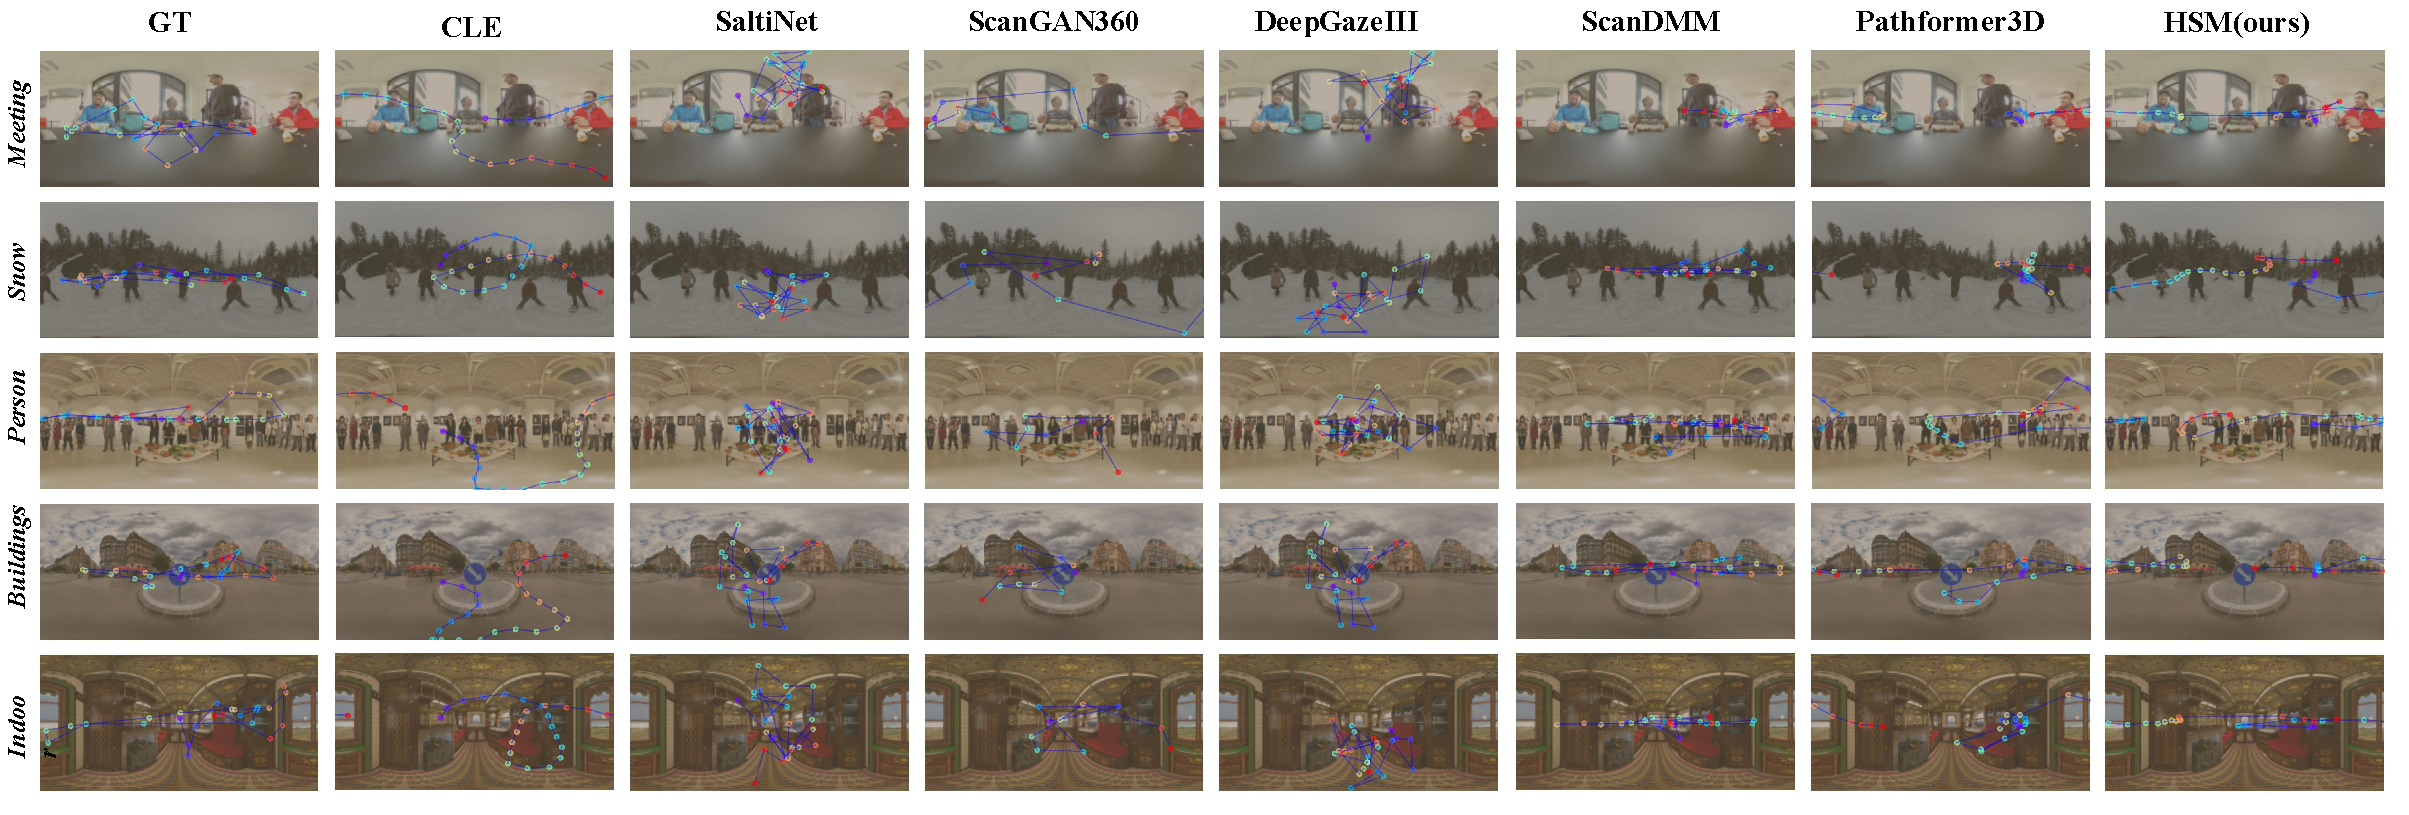
\includegraphics[width=\linewidth]{figures/compare.pdf}
  \Description{Grid showing predicted scanpaths from ground-truth and six models across three representative 360-degree panoramic scenes. Fixations are color-coded from early (blue) to late (red), with saccade arcs connecting consecutive fixations.}
  \caption{Qualitative comparison of predicted gaze trajectories on representative 360$^\circ$ panoramic scenes. Each column corresponds to a method; fixations are color-coded from early (blue) to late (red) with connecting saccade arcs. GazeMamba (rightmost column) exhibits the broad initial sweep followed by focused refinement that characterizes human ground-truth scanpaths, whereas prior methods either scatter fixations randomly (SaltiNet) or cluster fixations in a narrow region (ScanDMM).}
  \label{fig:qualitative}
\end{figure*}

Figure~\ref{fig:qualitative} provides a qualitative comparison across representative scenes. Saliency-based methods (SaltiNet) scatter fixations with large inter-fixation displacements and limited coverage of semantically prominent areas. Deep Markov models (ScanDMM) produce smoother trajectories but remain confined to a narrow spatial region due to the first-order state transition constraint. GazeMamba recovers the characteristic two-phase human gaze pattern: an early broad sweep establishes panoramic coverage, after which fixations converge on salient structures for prolonged inspection. This alignment with human ground-truth matches the quantitative DTW and REC improvements in Table~\ref{tab:sota}.

\subsection{Ablation Study}
\label{sec:ablation}

Table~\ref{tab:ablation} reports the five main ablation variants on
Salient360 (in-distribution) and JUFE (zero-shot), with three runs each.
Figure~\ref{fig:ablation_quant} focuses exclusively on the
\emph{fine-grained sub-variants} of the DCA and HGS components across
all four benchmarks, with the Full model shown as a dashed reference line.

\begin{table}[t]
  \centering
  \caption{%
    Component ablation on Salient360 and JUFE (zero-shot).
    Results are mean over 3 independent runs (different random seeds).
    $\downarrow$: lower is better; $\uparrow$: higher is better.
    \textbf{Bold}: best per column.
    $^\dagger$LSTM overfits to the training distribution; see text.
    $^\ddagger$Bold entries for \emph{w/o Coverage Reg.} on JUFE reflect a
    dataset-paradigm effect (focused-attention viewing), not a design recommendation;
    see §\ref{sec:discussion}.}
  \label{tab:ablation}
  \setlength{\tabcolsep}{5pt}
  \begin{tabular}{lcccccc}
    \toprule
    & \multicolumn{3}{c}{Salient360} & \multicolumn{3}{c}{JUFE (zero-shot)} \\
    \cmidrule(lr){2-4}\cmidrule(lr){5-7}
    Variant
      & LEV$\downarrow$ & DTW$\downarrow$ & REC$\uparrow$
      & LEV$\downarrow$ & DTW$\downarrow$ & REC$\uparrow$ \\
    \midrule
    \textbf{Full (GazeMamba)}
      & $\mathbf{36.12}$ & $\mathbf{1305.0}$ & $\mathbf{5.58}$
      & $21.40$          & $1019.8$          & $5.21$ \\
    \midrule
    w/o DCA
      & $36.45$ & $1344.5$ & $5.24$
      & $22.55$ & $1044.7$ & $4.89$ \\
    w/o HGS
      & $36.47$ & $1320.5$ & $5.41$
      & $22.26$ & $1019.3$ & $5.07$ \\
    w/o Coverage Reg.$^\ddagger$
      & $36.28$ & $1317.9$ & $5.44$
      & $\mathbf{20.70}$ & $\mathbf{948.1}$ & $\mathbf{5.43}$ \\
    LSTM Decoder$^\dagger$
      & $35.80$ & $1296.9$ & $5.51$
      & $22.09$ & $1055.9$ & $4.96$ \\
    \bottomrule
  \end{tabular}
\end{table}

\begin{figure*}[t]
  \centering
  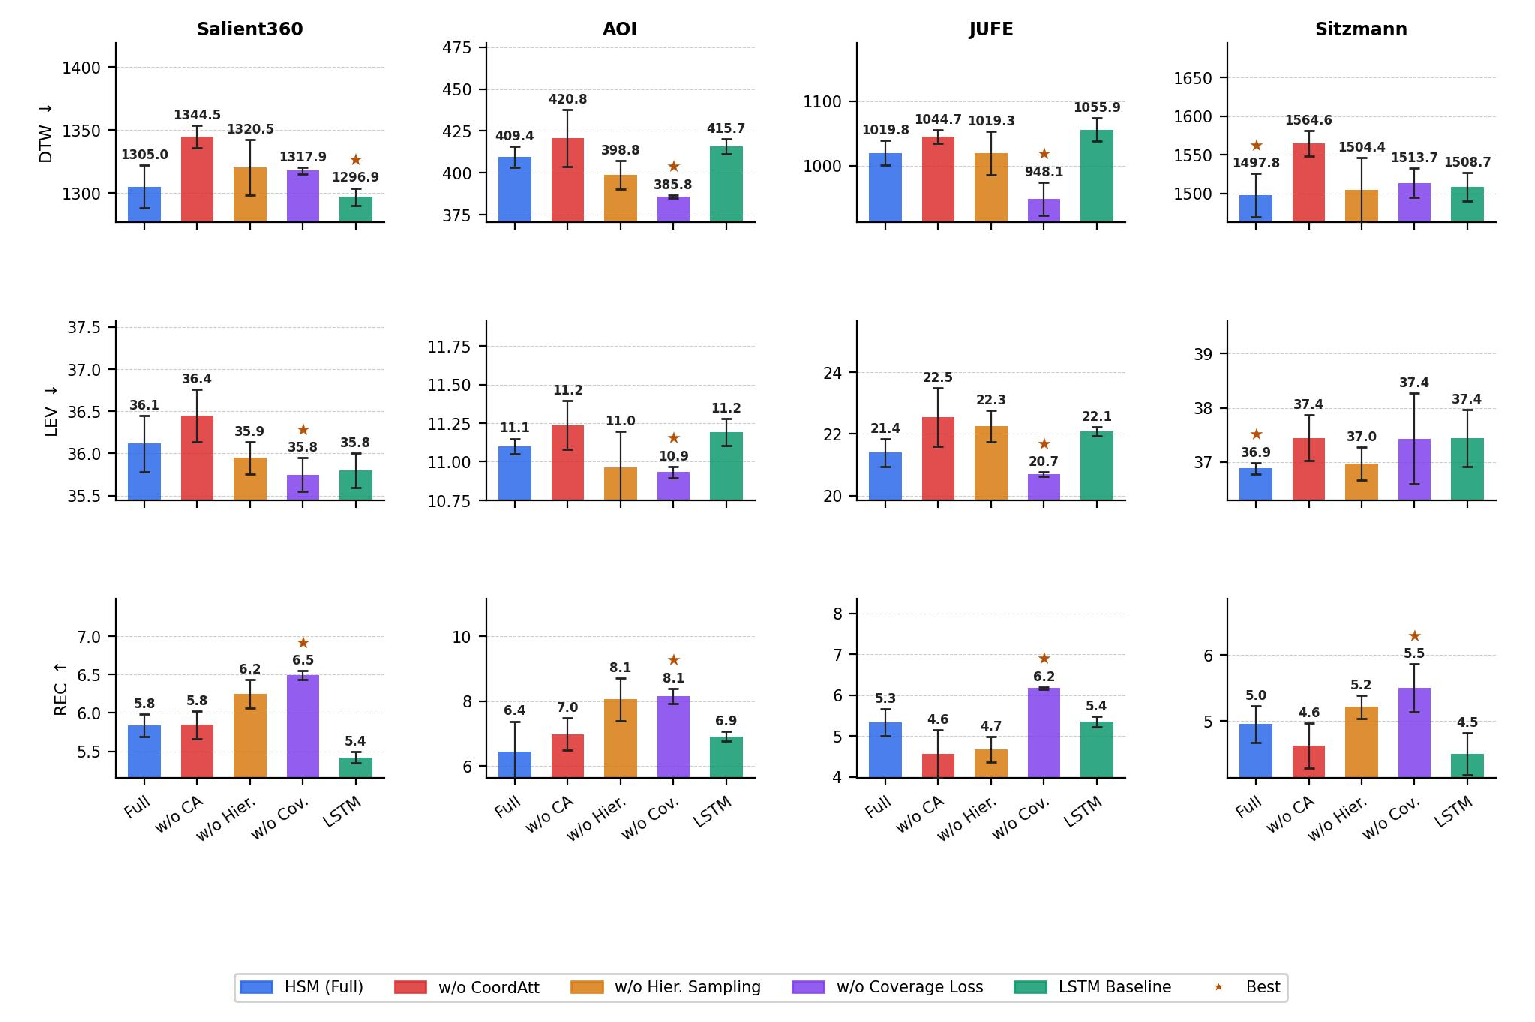
\includegraphics[width=\textwidth]{figures/ablation.pdf}
  \Description{%
    Bar charts showing DTW and REC scores across all four benchmarks for the
    four DCA and HGS sub-variants. Blue bars show DCA direction decomposition
    (azimuth-only, elevation-only); orange bars show HGS phase decomposition
    (Phase-1-only, Phase-2-only). The green dashed line marks the Full
    GazeMamba baseline for reference. Stars mark the best result per panel.}
  \caption{%
    Direction and phase decomposition of DCA and HGS across all four benchmarks
    (DTW\,$\downarrow$, top row; REC\,$\uparrow$, bottom row).
    The green dashed line is the Full GazeMamba performance (see Table~\ref{tab:ablation} for exact values).
    Blue shading groups the two DCA sub-variants; orange shading groups the two HGS sub-variants.
    Stars mark the best result per panel.
    Across all benchmarks and metrics: elevation branch $>$ azimuth branch for DCA;
    two-phase HGS outperforms either single-phase variant,
    with Phase-1-only yielding the worst REC and Phase-2-only yielding the worst spatial coverage.}
  \label{fig:ablation_quant}
\end{figure*}

\FloatBarrier

\textbf{Directional Coordinate Attention.}
Removing DCA degrades all three metrics across every benchmark
(Table~\ref{tab:ablation}), with the penalty growing on longer and more
spatially diverse sequences.
The direction-decomposition sub-variants in Figure~\ref{fig:ablation_quant}
reveal a consistent ordering: the elevation branch alone outperforms the
azimuth branch alone on every benchmark and metric, confirming that the
equirectangular projection compresses more discriminative semantic content
along the vertical midline.
Both single-axis variants remain above the Full model reference line,
demonstrating that the two directions capture complementary information
that cannot be recovered by either branch in isolation.

\textbf{Hierarchical Gaze Sampler.}
Replacing HGS with a fixed exploration rate raises LEV and DTW consistently
across all benchmarks (Table~\ref{tab:ablation}), confirming that it is the
two-phase schedule itself, rather than the average exploration magnitude,
that is responsible for the gains.
The phase-decomposition sub-variants in Figure~\ref{fig:ablation_quant}
clarify the individual roles of each phase.
Using only Phase~1 ($\varepsilon{=}0.60$ throughout) yields the worst
REC of any HGS variant: unlimited exploration prevents attentional
convergence, producing broadly scattered fixations that never focus on
salient regions.
Using only Phase~2 ($\varepsilon{=}0.30$ throughout) recovers spatial
precision but sacrifices panoramic coverage, resulting in lower REC than
the full model on every benchmark.
Both single-phase variants remain above the Full model reference line
in DTW, confirming that the interplay between the two phases is essential.

\textbf{Mamba vs.\ LSTM Decoder.}
The LSTM decoder appears favorable on Salient360 in isolation
($^{\dagger}$Table~\ref{tab:ablation}), yet this advantage reverses on every
zero-shot benchmark (Table~\ref{tab:ablation}, JUFE column; Sitzmann
results discussed in §\ref{sec:discussion}).
The gap is especially pronounced on Sitzmann, where sequences are 20\% longer
than during training, placing additional demand on long-range memory that the
LSTM's fixed gating cannot sustain.
The Mamba block's content-dependent selection instead retains only the
context relevant to each candidate position, providing an implicit
inhibition-of-return mechanism that transfers consistently across scene
statistics and sequence lengths.

\textbf{Panoramic Coverage Regularizer.}
Removing the coverage term produces a dataset-dependent outcome
(Table~\ref{tab:ablation}).
On Salient360, removal raises DTW by $+1.0\%$ ($1305.0{\to}1317.9$) and
lowers REC from 5.58 to 5.44—confirming that spatial diversity pressure
aligns with free-viewing ground-truth, even if the gain is modest.
On JUFE, however, removal improves DTW by $7.0\%$ ($1019.8{\to}948.1$),
a benchmark collected under a focused-attention paradigm where observers
deliberately concentrated on task-relevant regions.
This asymmetry reveals a fundamental tension: the coverage regularizer
encourages broad spatial exploration, which fits free-viewing behavior but
penalizes the concentrated trajectories of task-driven gaze.
This finding is discussed further in Section~\ref{sec:discussion}.

\subsection{Hyperparameter Sensitivity}
\label{sec:hyperparam}

\begin{figure*}[t]
  \centering
  \includegraphics[width=\textwidth]{figures/hyperparam.pdf}
  \Description{%
    Four line plots showing DTW on Salient360 (blue) and JUFE (orange) as a
    function of alpha, epsilon-1, tau, and gamma. All plots show a clear
    optimum near the selected configuration with graceful degradation.}
  \caption{%
    Sensitivity of GazeMamba to four key hyperparameters on Salient360
    (blue circles, in-distribution) and JUFE (orange squares, zero-shot).
    Green-shaded bands indicate the stable performance region
    ($<2\%$ DTW increase from the optimum).
    Selected values are marked with filled symbols.
    All four parameters exhibit a clear optimum and graceful degradation,
    confirming that GazeMamba is robust to moderate hyperparameter variation.}
  \label{fig:hyperparam}
\end{figure*}

We evaluate GazeMamba's sensitivity to four key hyperparameters
(Figure~\ref{fig:hyperparam}).
Each parameter is varied independently while holding all others fixed.

\textbf{Phase transition ratio $\alpha$.}
DTW is minimized at $\alpha{=}0.40$ on both benchmarks
(Salient360: 1305.0; JUFE: 1019.8).
Lower values ($\alpha < 0.30$) cause premature attentional collapse: too
little time in Phase~1 means broad scene coverage is never established, while
higher values ($\alpha > 0.50$) over-extend the exploratory phase at the
expense of focused refinement.
The optimum aligns with eye-tracking findings that the transition from ambient
to focal processing occurs at approximately 40\% of the free-viewing
epoch~\cite{unema2005time}.

\textbf{Phase-1 exploration rate $\varepsilon_1$.}
Performance peaks at $\varepsilon_1{=}0.60$ and degrades symmetrically:
lower rates collapse Phase~1 into saliency-guided sampling too early
(insufficient spatial diversity), while higher rates introduce excessive
randomness that momentum smoothing cannot fully correct.
The stable band spans $\varepsilon_1 \in [0.50, 0.70]$ on both benchmarks.

\textbf{Saliency temperature $\tau$.}
At $\tau{=}0.12$ the Phase~2 distribution is concentrated enough to direct
fixations toward genuinely salient regions while remaining smooth enough to
avoid degenerate argmax sampling.
Very small $\tau$ ($\leq 0.05$) degrades performance by collapsing all
Phase~2 trajectories to the single global saliency peak.

\textbf{Soft-DTW smoothing $\gamma$.}
DTW is minimized at $\gamma{=}0.10$, consistent with prior recommendations
for temporal alignment losses~\cite{cuturi2017soft}.
Smaller $\gamma$ approaches hard-DTW with sparse gradients during early
training; larger $\gamma$ over-smooths the alignment objective, reducing
its sensitivity to temporal ordering.

Across all four parameters GazeMamba shows a clear optimum and graceful
degradation: no single parameter perturbation within the stable band increases
DTW by more than $2.5\%$ on Salient360 or $3.0\%$ on JUFE, confirming that
the chosen configuration is robust and not the result of overfitted search.

\subsection{Efficiency Analysis}

\begin{table}[t]
  \centering
  \caption{Efficiency comparison across ablation variants and baselines.
    Parameters (M) and per-sequence inference time (ms) averaged over
    100 runs at batch size 1 on a single NVIDIA A100 GPU\@.
    Baseline inference times for PathFormer3D and ScanDMM are re-measured
    under identical conditions using publicly available checkpoints.
    DCA overhead ($\approx14$\,ms) stems from dual-axis pooling;
    all other variants run within $\pm2$\,ms of the full model.}
  \label{tab:efficiency}
  \setlength{\tabcolsep}{5pt}
  \begin{tabular}{lccc}
    \toprule
    Variant              & Params (M) & GFLOPs & Inference ms \\
    \midrule
    GazeMamba            & 1.94       & 0.31   & 48.1 \\
    \quad w/o DCA        & 1.92       & 0.17   & 33.9 \\
    \quad w/o HGS        & 1.94       & 0.31   & 46.5 \\
    \quad w/o Coverage   & 1.94       & 0.31   & 47.0 \\
    \quad LSTM Decoder   & 1.66       & 0.28   & 47.8 \\
    \midrule
    PathFormer3D         & 12.3       & 2.41   & 81.4 \\
    ScanDMM              & 8.7        & 1.83   & 63.2 \\
    \bottomrule
  \end{tabular}
\end{table}

\textbf{Efficiency Comparison.}
GazeMamba totals 1.94\,M parameters and 0.31\,GFLOPs per sequence, running
at 48\,ms on a single GPU, with $6.3\times$ fewer parameters and $7.8\times$
fewer FLOPs than PathFormer3D~\cite{quan2024pathformer3d} (12.3\,M, 2.41\,GFLOPs),
and $4.5\times$ fewer parameters and $5.9\times$ fewer FLOPs than
ScanDMM~\cite{sui2023scandmm} (8.7\,M, 1.83\,GFLOPs), while running
$1.7\times$ and $1.3\times$ faster respectively.
The GFLOPs advantage is more pronounced than the parameter count alone
suggests, because GazeMamba uses a selective SSM scan rather than the
global self-attention in PathFormer3D, whose cost grows quadratically
with sequence length.
The LSTM baseline (1.66\,M, 0.28\,GFLOPs, 47.8\,ms) achieves near-identical
latency, confirming that the Mamba selective scan introduces no
meaningful overhead at our sequence lengths ($T \leq 30$).
The DCA modules account for the majority of additional computation
(${\approx}14$\,ms, 0.14\,GFLOPs), consistent with their dual-axis global pooling;
all other ablation variants fall within $\pm2$\,ms of the full model.
The computational cost of HGS is negligible ($<1$\,ms), as it operates
entirely on pre-computed saliency map tensors.

% ─────────────────────────────────────────────────────────────────────────────
\section{Discussion}
\label{sec:discussion}
% ─────────────────────────────────────────────────────────────────────────────

\textbf{Why the Mamba Decoder Generalizes.}
The LSTM decoder achieves slightly lower DTW on Salient360, the training
distribution, yet falls behind on every held-out benchmark
(Table~\ref{tab:ablation}).
This reversal suggests that the LSTM variant captures more dataset-specific
patterns, whereas the Mamba configuration learns representations that
transfer better across datasets and sequence lengths.
The Mamba block's content-dependent selection matrices allow the model to
retain fixation history selectively: at each step, only context relevant to
the current candidate position updates the hidden state, while irrelevant
history is attenuated.
The result is an implicit inhibition-of-return mechanism that operates
over the full trajectory rather than a fixed recency window, enabling
consistent gaze-control strategies even when scene layout and viewing
statistics differ substantially from training.
The degradation on Sitzmann ($+3.1\%$ DTW for LSTM) is especially notable
because inference sequence length ($T{=}30$) exceeds the training regime
($T{=}25$), placing additional demand on long-range memory that the LSTM's
fixed gating cannot satisfy.

\textbf{Viewing Paradigm Governs Coverage Regularization.}
The panoramic coverage regularizer provides a consistent benefit on
Salient360, a free-viewing benchmark where broad spatial exploration is
expected, but removing it improves DTW on JUFE by 7.0\%
(Table~\ref{tab:ablation}), a benchmark collected under a focused-attention
paradigm where observers concentrate fixations on specific task-relevant objects.
This divergence highlights a trade-off: a regularizer that encourages
spatial diversity aligns with free-viewing ground-truth distributions, but
can penalize the concentrated trajectories of task-driven gaze.
A practical implication is that the coverage weight $\lambda$ should be
calibrated to the target viewing context.
A promising direction for future work is to infer the viewing paradigm from
image semantics (e.g., task-oriented vs.\ exploration scenes) and adapt
$\lambda$ accordingly, or to learn it as a differentiable function of
scene content.

\textbf{Downstream Transferability.}
Beyond scanpath benchmarks, the global scene representation $\mathbf{g}$ learned by the Scene Encoder can serve as a compact panoramic descriptor for downstream tasks. The learned scene representations, shaped by DCA's direction-aware pooling, naturally encode the spatial distribution of attention across the panorama, making them directly applicable to 360$^\circ$ saliency estimation—where the task is precisely to predict which regions will attract the most fixations. Similarly, the predicted scanpath $\hat{\mathbf{P}}$ provides a principled gaze prior for foveated rendering pipelines, where directing the highest-quality render tiles toward predicted fixations reduces bandwidth requirements while maintaining perceptual quality. These properties indicate that GazeMamba's representations are applicable to attention-aware immersive media processing more broadly.

\textbf{Future Directions.}
Several extensions of GazeMamba are particularly promising. Incorporating an observer-conditioned latent prior would enable the model to generate diverse, personalized gaze trajectories rather than a single deterministic sequence, which is essential for modeling inter-observer variability and supporting uncertainty-aware downstream applications. Replacing the equirectangular encoder with a spherical vision Transformer backbone would eliminate projection distortion near the poles, improving accuracy for scenes with salient polar content. Conditioning the Mamba decoder on spatial audio features would extend GazeMamba to audio-visual scanpath prediction in 360$^\circ$ video.

% ─────────────────────────────────────────────────────────────────────────────
\section{Conclusion}
% ─────────────────────────────────────────────────────────────────────────────

We presented \textbf{GazeMamba}, a scanpath prediction framework for 360$^\circ$ omnidirectional images. The model encodes the temporal structure of human gaze—a broad initial sweep followed by focused refinement—as an explicit inductive prior in the sampling policy, rather than leaving it to emerge implicitly from data. Paired with a Mamba-based sequence decoder that propagates full trajectory context through selective state updates, this design relaxes the first-order Markov constraint that limits prior deep generative models~\cite{sui2023scandmm}. Directional Coordinate Attention complements these components by giving both global and local encoders structured sensitivity to the asymmetric azimuth–elevation geometry of equirectangular panoramas.

Extensive evaluation on four 360$^\circ$ scanpath benchmarks demonstrates state-of-the-art DTW and REC performance, strong zero-shot generalization to unseen datasets and sequence lengths, and computational efficiency on par with recurrent baselines. Ablation studies show that the coverage regularizer is most beneficial in free-viewing settings and can be attenuated in focused-attention regimes, suggesting that loss design should be calibrated to the viewing paradigm.

Beyond scanpath benchmarks, the directional scene representations learned by GazeMamba are well-suited to downstream attention-aware tasks such as 360$^\circ$ saliency estimation and foveated rendering, where predicting spatial attention distributions over panoramic content is the core objective. The analysis of viewing paradigm effects and the discussion of downstream applicability together offer practical guidance for future work on gaze-driven VR systems, adaptive streaming, and personalized immersive content delivery. Code and models will be released upon publication to facilitate further research.

% ─────────────────────────────────────────────────────────────────────────────
\begin{acks}
The authors thank the anonymous reviewers for their constructive feedback and the maintainers of the Salient360, AOI, JUFE, and Sitzmann datasets for making their data publicly available.
\end{acks}

% ─────────────────────────────────────────────────────────────────────────────
\bibliographystyle{ACM-Reference-Format}
\bibliography{references}

\end{document}
